\section{Background and Related Work}

\subsection{Observability}

As software continues to scale into Internet-scale systems that have complex interactions with other
applications and underlying hardware, so too does their failure domain: distributed systems become
pathologically unpredictable, as performance regressions and partial failures can arise anywhere
from the network \ref{8-fallacies} to the underlying storage system to competing
processes on the same machine \ref{noisy-neighbors}. Thus, in order to develop and maintain robust
systems, developers increasingly rely on observability systems to monitor system health and
performance (ref: DSO) (ref: SRE book).

\subsubsection{Existing Systems}

Current observability systems focus primarily on three types of telemetry data: logs, metrics, and
traces (collectively termed the ``Three Pillars of Observability'' (ref: pillars of observability)):

% TODO: maybe condense this a lot?
\begin{itemize}
    \item Logs are semi-structured or unstructured strings added into applications by developers to
        expose highly granular information with local context. For example, logs could include stack
        traces from software bugs or exceptions, or database access events with associated contexts
        to debug performance regressions. Existing systems include ElasticSearch (ref: ES) and CLP
        (ref: CLP) for log processing.
    \item Metrics provide quantitative measurements of system performance and availability at a
        specific point in time. Metrics can be \textit{counters} that represent cumulative,
        monotonically increasing values (e.g. HTTP requests received, GC collections executed),
        gauges to model system state (e.g. CPU/memory usage, machine availability), or histograms of
        observed values (e.g. request latencies) (ref: metric types). Existing systems include
        Prometheus (ref: Prometheus) and M3DB (ref).
    \item Distributed traces follow program execution flow and often resemble call graphs. For
        example, a trace of an HTTP request might show the internal backend and database functions
        invoked to satisfy the request. Existing systems include Jaeger (ref: Jaeger) and Zipkin
        (ref: Zipkin).
\end{itemize}

Current observability systems have expanded into robust distributed systems themselves, with some
like InfluxDB (ref) and ClickHouse (ref) capable of handling general time-series data. However,
these systems often fail to capture the underlying root cause of a system anomaly (ref: doordash bpf).

Concretely, consider a performance engineer investigating a performance regression in a
microservices application. Via application-level aggregated metrics, the engineer can identify a
system bottleneck from the backing RocksDB application by identifying spiking tail latency metrics;
from there, they can use traces to pinpoint the specific problematic function (say, \texttt{pread64}
within the \texttt{GET} operation). However, although the engineer now knows \textit{where} the
system bottleneck arises, they do not know \textit{why} it is occuring. 

To analyze the root cause of performance regressions like this, developers must turn to
high-fidelity telemetry (HFT) data.

\subsubsection{High-Fidelity Telemetry (HFT) Data}

HFT data refers to data generated from kernel events with a much higher level of granularity; some
examples are page cache evictions or CPU scheduler events. As HFT data is generated within the
kernel, they contain comprehensive information about the context from which it originated, such as
the specific inode and device number on which a page cache eviction occurs, or which \texttt{pid}s
are being scheduled and their priority levels. Using HFT data, developers can interactively
investigate various system events for anomalies, and identify the root cause for system anomalies.

The amount of HFT data available to be collected can be orders of magnitude greater than that of
traditional telemetry data, due to the higher granularity of each individual data point. As an
illustrative example, in a RocksDB application, gathering HFT data on \texttt{pread64} syscall
\textit{invocations} alone can produce millions of events per second; the amount could significantly
increase if other events were instrumented (such as CPU scheduling, page cache events, or memory
allocations). As such, HFT data is often summarized as some aggregate statistic, such as average,
histogram buckets, or quantiles.

HFT data can prove invaluable in identifying performance regressions. In the above example, an
engineer can use HFT data to formulate a hypothesis about the root cause, and monitor various kernel
events. For instance, they could correlate system call latency with other kernel events like page
cache events, and identify that a competing process is causing repeated page cache evictions; from
then, they can appropriately handle the competing process (e.g. by re-scheduling it to a different
machine).

HFT data collection's use case of anomaly debugging imposes strict requirements. Especially since
this functionality is often injected at program hot paths or in systems under high load, HFT data
collection programs must incur negligible overhead and remain performant, even under intense
resource pressure. Moreover, due to the ever-evolving nature of distributed applications, programs
must be dynamic, flexible, and simple to generate. In addition, HFT data must be as complete as
possible, as sparse data sampling can result in key anomalous events frequently being dropped (ref:
sampling bad). Finally, HFT data output should be exposed through accessible interfaces, as often
their results must be post-processed for offline analysis.

To support HFT data collection, various tracing technologies have been developed, either within the
Linux kernel or as research systems. However, these tools often introduce prohibitive overhead, emit
insufficient contextual information, or are difficult to develop and adapt, making it unsuitable to
handle HFT data collection's requirements.

Event profilers like \texttt{perf} (ref), \texttt{ftrace} (ref), \texttt{DTrace} (ref), and
\texttt{SystemTap} trace kernel events and emit information at various degrees of granularity.
However, these systems often incur prohibitive overhead costs that make them unsuitable for
production systems (ref: function duration with ftrace, Hubble paper). For example, the
\texttt{perf} subsystem uses interrupt-based sampling, which introduces costly context switches and
branch misses (ref: perf tutorial, perf analysis modern CPUs). These systems must thus resort to
aggressive sampling, causing key events to be dropped. Moreover, these utilities emit data in ad-hoc
formats, forcing developers to write custom post-processing scripts and manually manage result
storage.

Other tracing instrumentation tools like Magpie (ref), KUTrace (ref), Nanoscope (ref), Shim (ref),
and Hubble (ref) generate HFT data through lightweight instrumentation. Although these systems are
performant, they are purpose-specific: Nanoscope and Hubble specifically target the Android runtime,
KUTrace is a Linux kernel tracing patch, and Shim primarily targets hardware performance counters
and signals. As a result, they are not suitable for general-purpose application tracing, and
interacting with the generated data also requires manual post-processing.

The Linux kernel exposes tracepoints (ref) and kprobes (ref), allowing developers to instrument
specific kernel instructions or events with low overhead. However, regular tracepoints can only be
interacted with by writing user-space code to process a pre-determined context, and kprobes
introduce significant safety risks, as faulty programs could crash the kernel (ref: guts of
kprobes). Both solutions require developers to intimately understand the kernel tracing
infrastructure.

The fragmentation of various tracing utilities and output formats poses real difficulties for
developers trying to debug anomalies. In a case study by Cloudflare (ref: blog 1, blog 2) debugging
a latency spike, five separate custom \texttt{SystemTap} scripts were required, alongside
\texttt{netstat} and \texttt{tcpdump}, in order to identify the root cause. Without a structured
utility to process results, developers are forced to manually inspect and debug system regressions.

\subsection{eBPF}

In recent years, a novel kernel technology, the extended Berkeley Packet Filter (eBPF), has opened
a promising new approach to HFT data collection by providing a minimalistic sandboxed ``virtual
machine'' (ref: eBPF VM patch, tc classifier programmable) to safely execute custom user programs,
allowing developers to safely and efficiently extend kernel capabilities without kernel patches or
modules (ref: what is eBPF).

The Berkeley Packet Filter (BPF or cBPF), introduced in 1992, originated as a subsystem that allowed
userspace programs to execute in a limited kernel virtual machine at specific network stack hook
points (ref: BSD packet filter). Its functionality was later expanded into its current state, eBPF,
with an expanded instruction set architecture that closely maps to native CPU instructions, a JIT
compiler, a verifier to ensure program safety, persistent state via BPF maps, and support for the
LLVM toolchain for compilation (ref: what is eBPF). Most importantly, eBPF expanded to arbitrary
kernel events, allowing custom programs to hook into events ranging from the network stack, to Linux
Security Modules (LSM), to internal tracing technologies, such as (raw) tracepoints,
\texttt{u[ret]probes/k[ret]probes}, and \texttt{fentry/fexit}. This expanded feature set has enabled
highly performant and extensible HFT data collection. (Beyond tracing, eBPF has also been used for
efficient in-kernel packet processing (ref: XDP), CPU scheduling (ref: Ghost), and kernel bypass
storage functions (ref: XRP)).

\begin{quote}
From here on, the term ``eBPF'' will be used interchangeably with ``BPF'', as cBPF is no longer
used.
\end{quote}

\subsubsection{eBPF System Architecture}

\begin{figure}[htpb]
    \centering
    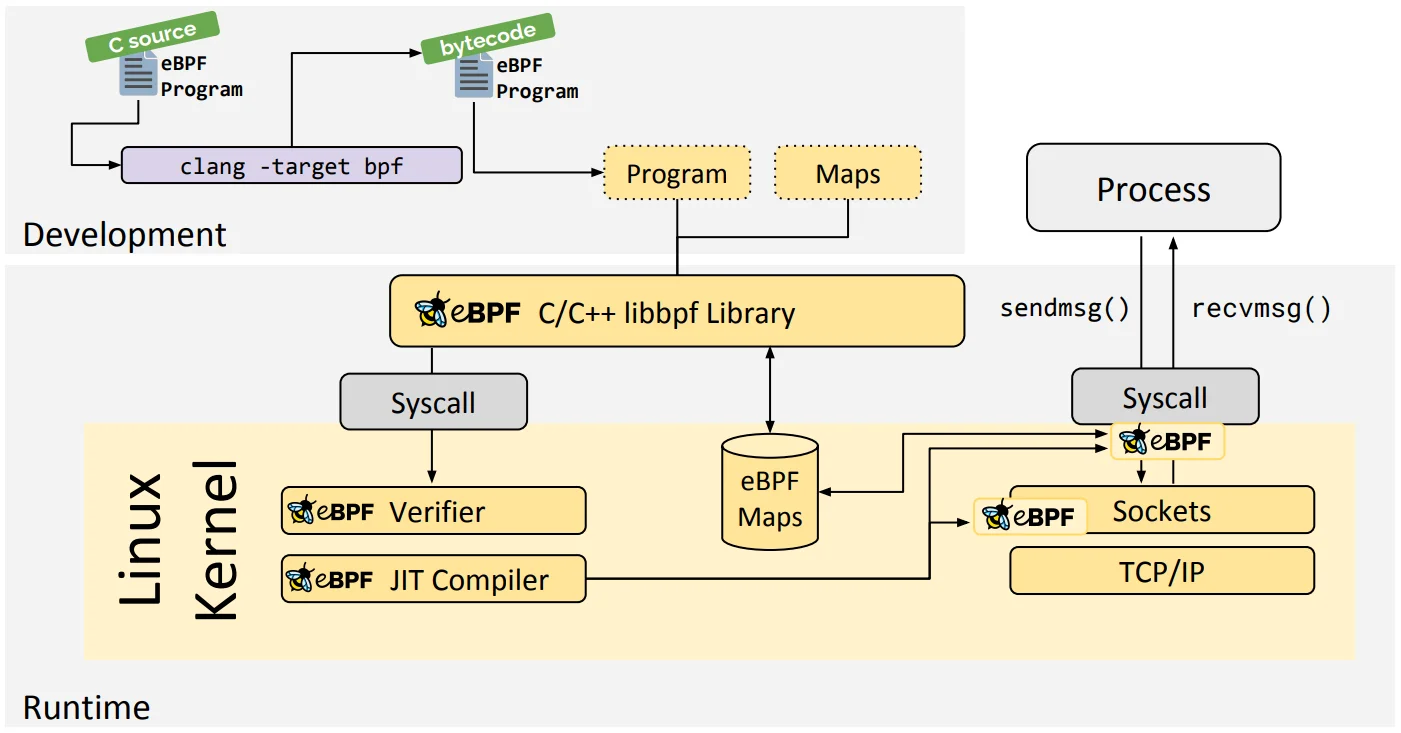
\includegraphics[width=0.8\textwidth]{diagrams/ebpf-architecture.png}
    \caption{eBPF Architecture using libbpf (from (ref: what is eBPF))}
    \label{fig:bpf-arch}
\end{figure}

eBPF consists of multiple components (see Figure \ref{fig:bpf-arch}):

\begin{itemize}
    \item Engineers write custom eBPF program code in essentially a subset of C, albeit with
        important exceptions: for example, unbounded or dynamically sized loops are forbidden,
        helper function calls could not have more than 5 arguments (non-inlined helper functions
        were not supported until Linux v4.9 (ref: bpf function calls)), the stack size is restricted
        to 512 bytes, and a maximum of 1 million BPF instructions are allowed (prior to Linux v5.1,
        this limit was a mere 4096 instructions (ref: increase complexity limit)). eBPF C disallows
        dynamic memory; instead, developers must use BPF maps to persist state across program
        executions or use memory beyond the 512B limit. BPF maps also enable communication between
        user and kernel space. eBPF source code files can contain multiple eBPF ``programs'' for
        different kernel events, specified with a \texttt{SEC} macro before function definitions.

        As an example, Figure \ref{code:pread64-unopt} contains a standard BPF program to instrument
        the \texttt{pread64} system call.
\begin{figure}
\begin{lstlisting}[language=C]
#include "vmlinux.h"
#include <bpf/bpf_core_read.h>
#include <bpf/bpf_helpers.h>
#include <bpf/bpf_tracing.h>

typedef struct {
    u64 time;
    u64 fd;
    u64 cpu;
    u64 count;
} raw_pread_t;

#define RB_MAX_ENTRIES (1024 * sizeof(raw_pread_t))
struct {
    __uint(type, BPF_MAP_TYPE_RINGBUF);
    __uint(max_entries, RB_MAX_ENTRIES);
} ring_buf_pread_query SEC(".maps");

SEC("tp/syscalls/sys_enter_pread64")
u32 pread_query(struct trace_event_raw_sys_enter* ctx) {
    raw_pread_t* q = bpf_ringbuf_reserve(
        &ring_buf_pread_query,
        sizeof(raw_pread_t),
        0
    );
    if (!q) {
        bpf_printk("failed to allocate space in ring buffer");
        return 1;
    }
    q->time = bpf_ktime_get_ns();
    q->fd = ctx->args[0];
    q->cpu = bpf_get_smp_processor_id();
    q->count = ctx->args[2];
    bpf_ringbuf_submit(q, 0);
    return 0;
}

char LICENSE[] SEC("license") = "Dual BSD/GPL";
\end{lstlisting}
\caption{A standard \texttt{pread64} tracing BPF program.}
\label{code:pread64-unopt}
\end{figure}

        Once written, these programs are compiled into eBPF bytecode using the LLVM/\texttt{clang}
        toolchain, which generates an object file containing all defined eBPF programs and map
        definitions. 

    \item When the program is ready to be inserted into the kernel, eBPF bytecode is passed to the
        \texttt{bpf} system call (ref: bpf system call), which loads the program into the kernel. As
        the \texttt{bpf} syscall operates on compiled program bytes, working with compiled programs
        can prove difficult (e.g. to edit global variables or map definitions before runtime); thus,
        a higher-level wrapper library, \texttt{libbpf}, was introduced (in the figure, the
        higher-level \texttt{libbpf} library is for C/C++; however, support for other languages,
        like Go and Rust, also exist).

    \item The \texttt{bpf} syscall passes the eBPF bytecode to the eBPF verifier, which ensures the
        safety and soundness of eBPF programs, rejecting any program that might potentially be
        unsound by checking for guaranteed termination and memory safety. The verifier traverses
        through all program paths, using heuristics to prune potential program branches (ref: static
        analysis), and maintaining a DAG to ensure bounded loop termination and other CFG validation
        (ref: linux eBPF verifier doc). On each instruction, the verifier maintains a range of
        possible values for each register value, ensuring that they are valid (e.g. a memory access
        for register $R$ is in the allowed range). Only after verifying that all program
        instructions are sound does the kernel accept the eBPF program.

        Because dynamic memory access adds significant complexity, the eBPF verifier requires that
        such access is known at verification time. In particular, BPF maps, stored in kernel space
        and represented with file descriptors, must have their \texttt{fd}s embedded in the
        \texttt{BPF\_LD\_IMM64} instruction; and function calls must be to either a constant
        function definition or a pre-defined BPF ``helper function'' (ref: bpf helpers) that exposes
        additional kernel functionality (in other words, function pointers are disallowed in BPF
        programs, except in certain contexts like in the \texttt{bpf\_for\_each\_map\_elem} helper).
    \item After verification, the program is injected into the designated hook point; then, every
        time the kernel event occurs, the program runs within that context. BPF programs then
        communicate with userspace programs by writing data to the shared BPF maps, on which
        userspace programs can then invoke syscalls to retrieve the data from the kernel.
\end{itemize}

\subsubsection{eBPF as a HFT Data Collection Tool}

Given its architecture, eBPF is uniquely suited to handle HFT data collection. 

First, the eBPF verifier guarantees that custom programs are safe to run, and that users have
requisite permissions. Thus, buggy or unsafe programs are rejected before being loaded and executed.
This exists in stark contrast to existing technology, where software bugs can crash the entire
kernel. For example, it is possible to hook into arbitrary kernel instructions for tracing via
kprobes (ref: kprobes), but errors in the probes would crash the kernel (ref: guts of kprobes).

Second, expressive eBPF programs can run with high performance, minimal overhead, at a level
acceptable in production environments. Because eBPF programs are provably sound, they can inject
\textit{custom} code into exclusive kernel tracing infrastructure, like
\texttt{fentry}/\texttt{fexit} and tracepoints (which do not offer the same expressiveness to other
userspace tracing methods). Moreover, the eBPF JIT compiler transparently compiles eBPF bytecode
into native machine instructions, allowing cross-platform efficient execution with almost trivial
overhead. As a concrete example, BPF programs attached to the XDP hook point can process over 24
million packets per second (ref: XDP).

Third, eBPF programs can be dynamically loaded and modified during application runtime, allowing
instrumentation without disrupting existing systems. As applications evolve and change, eBPF
programs can be seamlessly modified to accommodate the new changes; similarly, the programs
themselves may be extended with additional functionality without disrupting existing systems. This
allows teams to decouple application development and monitoring, lifting the burden off engineers
during the development process.

\subsection{eBPF Development Challenges}

Despite its various benefits, onboarding into the eBPF ecosystem and developing performant,
verifiable eBPF programs remains a significant challenge.

First and foremost, the eBPF verifier can reject seemingly sound BPF programs. In some cases, the
verifier is overly restrictive, rejecting programs due to an inability; in other cases, the verifier
encounters constructs outside of eBPF's current supported feature set, causing it to reject
programs. To complicate matters, the verifier's error messages deal primarily with eBPF bytecode and
the virtual registers, and can be uninformative at best and misleading at worst. We consider three
illustrative examples:

\begin{enumerate}
    \item The eBPF program in Figure \ref{code:fail-1} accumulates up to
        \texttt{RINGBUF\_MAX\_ENTRIES} context values, then emits them to the ring buffer.
\begin{figure}[htpb]
\begin{lstlisting}[language=C]
#include "vmlinux.h"
#include <bpf/bpf_core_read.h>
#include <bpf/bpf_helpers.h>
#include <bpf/bpf_tracing.h>
#define RB_MAX_ENTRIES (1<<18)
struct {
    __uint(type, BPF_MAP_TYPE_RINGBUF);
    __uint(max_entries, (RB_MAX_ENTRIES * sizeof(u64)));
} rb SEC(".maps");
u64 global_count = 0;

SEC("tp/syscalls/sys_enter_pread64")
u32 pread_query(struct trace_event_raw_sys_enter *ctx) {
    u64 count = global_count;
    global_count += 1;
    if (count >= RB_MAX_ENTRIES) {
        u64 *records = bpf_ringbuf_reserve(&rb,
            count * sizeof(u64), 0);
        if (records != NULL) {
          bpf_ringbuf_submit(records, 0);
        }
        global_count = 0;
    }
    return 0;
}
\end{lstlisting}
\caption{An example program that accumulates values before emitting to user-space.}
\label{code:fail-1}
\end{figure}

    This fails the eBPF verifier with the error: 
\begin{lstlisting}
// ... more output ... //
R1_w=inv262144 R2_w=inv(id=0,umin_value=262144) R10=fp0
; u64 *records = bpf_ringbuf_reserve(&rb, count*sizeof(u64), 0);
7: (67) r2 <<= 3
8: (b7) r6 = 0
12: (85) call bpf_ringbuf_reserve#131
R2 is not a known constant'
\end{lstlisting}
    From a developer standpoint, we can verify that the BPF program is safe to execute, as
    \texttt{global\_count} will only ever be at most \texttt{RB\_MAX\_ENTRIES}; and because we
    assign \texttt{global\_count} to a local variable \texttt{count}, this would not pose an issue
    with other concurrently executing processes. However, because the verifier operates on variable
    ranges with only individual execution-level context, it is unable to verify the logic.

    To remedy this, a line manually setting \texttt{count = RB\_MAX\_ENTRIES} would be required.
    This kind of massaging to appease the verifier is common in eBPF programs.

    \item The eBPF code snippet in Figure \ref{code:fail-2} attempts to copy over data from one
        buffer to another (both stored as global variables).
\begin{figure}[htpb]
\begin{lstlisting}[language=C]
#define BUF_SZ (1 << 16)
u8 src[BUF_SZ] = {0};
u8 dst[BUF_SZ] = {0};
// ... additional code ... //
__builtin_memcpy(dst, src, sizeof(src));
\end{lstlisting}
    \caption{An eBPF code snippet that copies values from one eBPF array to another.}
    \label{code:fail-2}
\end{figure}
    On program load, the BPF verifier emits the message, \texttt{error: A call to built-in
    function 'memcpy' is not supported}, and rejects the program, even though the clang instrinsic
    \texttt{\_\_builtin\_memcpy} is supported in eBPF environments. After much digging, the cause of
    this error is because the stack size is limited to 512B, and so builtin memory operations fail
    when operating on structs larger than that (ref: iovisor bcc memset).

    To remedy this, the \texttt{memcpy} would have to be replaced with a call to
    \texttt{bpf\_probe\_read\_kernel}, which introduces an additional overhead of memory copying and
    runtime safety checks.

    \item The eBPF code snippet in Figure \ref{code:fail-3} attempts to declare a map of $2^{20}$
        elements.
\begin{figure}[htpb]
    \centering
\begin{lstlisting}[language=C]
struct {
    __uint(type, BPF_MAP_TYPE_HASH);
    __type(key, u64);
    __type(value, u64);
    __uint(max_entries, (1 << 20));
} map SEC(".maps");
\end{lstlisting}
    \caption{An eBPF code snippet attempting to initialize a large map.}
    \label{code:fail-3}
\end{figure}

    On program load, the BPF verifier emits the error message:
\begin{lstlisting}
Error in bpf_create_map_xattr(prog.bss):Argument list too long(-7). Retrying without BTF.
map 'prog.bss': failed to create: Argument list too long(-7)
libbpf: failed to load object 'prog_bpf'
libbpf: failed to load BPF skeleton 'prog_bpf': -7
\end{lstlisting}

    After much investigation, the root cause for this is because \texttt{bpf\_create\_map} invokes
    the internal kernel \texttt{kmalloc} (ref: kernel code), which on most machines has a limit of
    4MB; thus, maps larger than that are rejected. Unfortunately, the actual error message provides
    little insight into BPF's limitations, with no specific indication that map sizes have this
    fixed limit.
\end{enumerate}

There are some important takeaways from this. First, due to the verifier's limited
individual-execution scope, developers must frequently appease the verifier by adding redundant
checks and redundant accesses, incurring real performance hits; otherwise, sound programs would be
rejected. Second, the verifier often emits obscure or misleading error messages, forcing the
developer to manually test different parts of their program, scour online discussion forums, or
investigate the BPF kernel itself to pinpoint the cause. These combined can significatly impedes
developer workflows.

Beyond the verifier, the eBPF ecosystem also can hinder developers. Due to its volatile and evolving
interface, many APIs are unstable and are frequently changed; moreover, online documentation often
fails to keep up with recent developments, resulting in misleading and outdated information, or even
a complete lack thereof, forcing developers to resort to kernel patch updates or mailing lists. As
concrete examples, the \texttt{bpf-helpers} manpage explicitly refers developers to the kernel
source for an up-to-date list of helper functions (ref: bpf-helpers manpage); and simple questions
such as ``Can I clear a BPF map within a BPF program?'', ``How can I pin BPF maps to share across
programs?'', and ``Can I use this BPF helper function at this kernel event?'' require deep
exploration of online resources or even the kernel source (ref: pin patch, iovisor-dev mailing
list).

Even with a BPF program that passes the BPF verifier, developers must also be familiar with kernel
environments, which operate with further restrictions (for instance, floating point operations are
not supported). Moreover, due to the eBPF architecture, it is easy to develop inefficient programs
without a deep knowledge of eBPF subtleties.

For example, prior work (ref: eBPF traffic sketching) has explored different memory access patterns
in eBPF for data structure design, comparing four different ways to represent a 2D $R\times C$ array
(an array map with one $R\times C$-sized array, an array map with $R$ entries of $C$-sized arrays,
an array map with $R\times C$ entries, and an array of array map with $R$ array maps, each with $C$
entries). Perhaps surprisingly, different access patterns incur varying amounts of overhead (Figure
\ref{fig:array-access}).

\begin{figure}[htpb]
    \centering
    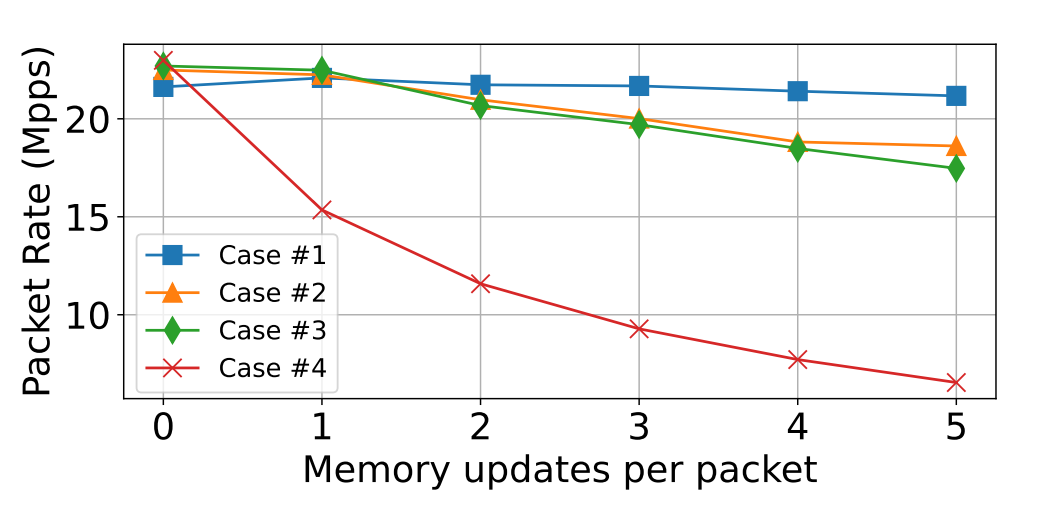
\includegraphics[width=0.8\textwidth]{diagrams/ebpf-array-accesses.png}
    \caption{Different methods of array accesses (from (ref: eBPF traffic sketching)).}
    \label{fig:array-access}
\end{figure}

Beyond these cases, eBPF structures often incur hidden synchronization overhead due to its
concurrent execution environment; this can be resolved with different per-CPU and task-local
constructs that reduce overhead at the expense of higher developer complexity, but only if
developers are intimately aware with the environment (ref: fast and slow blogpost).

\subsection{Related Work}

To ease BPF development, a robust ecosystem providing higher-level wrappers around BPF internals has
emerged.

\subsubsection{\texttt{bcc}}

One of the most popular development frameworks is the BPF Compiler Collection, or \texttt{bcc} (ref:
bcc). Its architecture is displayed in Figure \ref{fig:bcc-architecture}.

\begin{figure}[htpb]
    \centering
    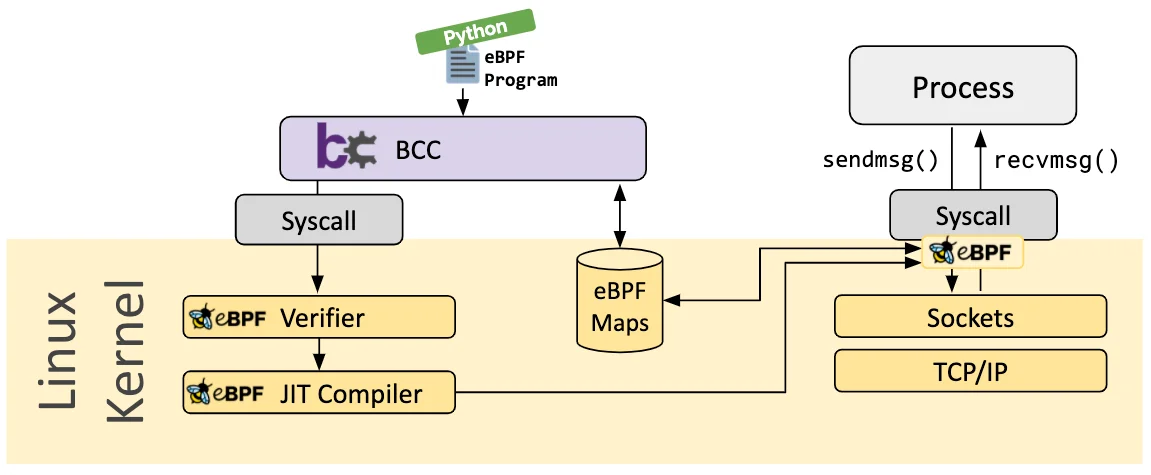
\includegraphics[width=0.8\textwidth]{diagrams/bcc-architecture.png}
    \caption{The BCC eBPF Architecture.}
    \label{fig:bcc-architecture}
\end{figure}

Development follows a similar workflow to raw BPF program development, with some key additions:
\begin{itemize}
    \item \texttt{bcc} introduces a higher-level Python/Lua frontend for communicating with BPF
        programs and the \texttt{bpf} syscall, simplifying access and modification of shared BPF
        maps, global variables, and other program configuration options.
    \item \texttt{bcc} adds additional macros and pre-processing steps before loading BPF code,
        simplifying section/program type macros, map definitions and accesses, and certain BPF
        helper functions.
\end{itemize}

Despite its simplified development environment, however, \texttt{bcc} runs into numerous challenges.
First, although some constructs are simplified, the actual BPF program---the key instrumentation
code---must still be written in BPF C; the program text must then be embedded into the Python
frontend and loaded, before the program can begin tracing. For example, the BCC program in Figure
\ref{code:bcc-example} (from (ref: disksnoop)) traces disk block IO requests.
\begin{figure}[htpb]
\begin{lstlisting}[language=C]
# load BPF program
b = BPF(text="""
#include <uapi/linux/ptrace.h>
#include <linux/blk-mq.h>

BPF_HASH(start, struct request *);

void trace_start(struct pt_regs *ctx, struct request *req) {
    u64 ts = bpf_ktime_get_ns();
    start.update(&req, &ts);
}

void trace_completion(struct pt_regs *ctx, struct request *req) {
    u64 *tsp, delta;
    tsp = start.lookup(&req);
    if (tsp != 0) {
        delta = bpf_ktime_get_ns() - *tsp;
        bpf_trace_printk("%d %x %d\n",
            req->__data_len, req->cmd_flags, delta / 1000);
        start.delete(&req);
    }
}
""")

b.attach_kprobe(event="blk_start_request", fn_name="trace_start")
b.attach_kprobe(event="blk_account_io_done", fn_name="trace_completion")
// Additional processing code...
\end{lstlisting}
\caption{A BCC \texttt{disksnoop} script (from (ref: disksnoop))}
\label{code:bcc-example}
\end{figure}

The fundamental burden of developing the BPF code is still the developer's responsibility.
Furthermore, \texttt{bcc}'s various abstractions can additionally hinder development, as it uses its
own naming conventions, hides various initialization and auto-generated struct definitions, and uses
a non-standard object-oriented version of C that often differs from internal kernel operations (ref:
bcc to libbpf). As a result, the standard \texttt{libbpf} development environment is often
preferred.

\subsubsection{Cilium}

Cilium is a cloud-native monitoring, networking, and security platform for managing containerized
Kubernetes environments (ref: Cilium). Cilium provides useful utilities out-of-the-box, exposing
Prometheus metrics for container and pod health, and abstracts away much of the complexity of eBPF
by using it only internally. 

However, its focus is on cloud, containerized environments, with functionality geared primarily
towards networking and security; as such, its monitoring utilities are mainly for those purposes,
and due to its higher-level nature, exposes more aggregate metrics on system health, rather than the
high-granularity HFT data needed for root cause analysis.

In addition to the Cilium platform, it provides a Go frontend wrapping eBPF functionality (much like
\texttt{bcc}), simplifying management of BPF maps and programs from user-space. However, like
\texttt{bcc}, Cilium also relies on embedded eBPF programs. Thus, the burden of developing BPF
instrumentation programs still lies with the developer.

\subsubsection{\texttt{bpftrace}}

\texttt{bpftrace} (ref: bpftrace) provides the most high-level interface over eBPF, exposing a
tracing language similar to DTrace (ref: DTrace). Its architecture is displayed in Figure
\ref{fig:bpftrace-architecture}.

\texttt{bpftrace} takes in a script written in its higher-level language, parses it into an AST,
converts it into LLVM IR, then hooks into the LLVM toolchain to compile into eBPF bytecode. The
compiled program is then automatically loaded into the kernel.

\begin{figure}[htpb]
    \centering
    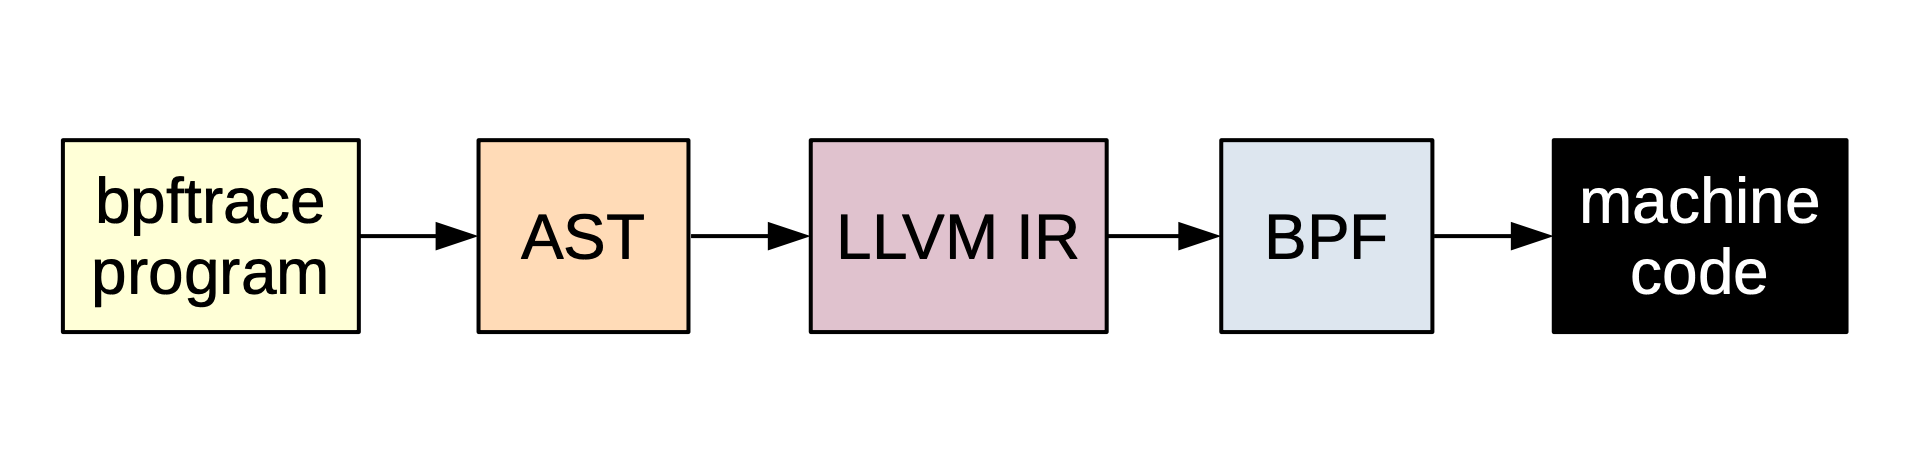
\includegraphics[width=0.8\textwidth]{diagrams/bpftrace-architecture.png}
    \caption{\texttt{bpftrace} architecture (from (ref: BPF Internals))}
    \label{fig:bpftrace-architecture}
\end{figure}

\texttt{bpftrace}, in many ways, provides a sufficiently high-level abstraction over BPF, enabling
developers to write custom tracing scripts without writing BPF C. However, its design contains
two problems. First, \texttt{bpftrace} is a fundamentally procedural language; thus, developers must
explicitly enumerate program steps, grounding development into the same procedural
programming required for BPF C.

Concretely, consider the \texttt{bpftrace} program in Figure \ref{code:bpftrace-ex}, which
instruments the \texttt{open} syscall.

\begin{figure}[htpb]
\begin{lstlisting}[language=C]
tracepoint:syscalls:sys_enter_open,
tracepoint:syscalls:sys_enter_openat
{
    @filename[tid] = args.filename;
}
tracepoint:syscalls:sys_exit_open,
tracepoint:syscalls:sys_exit_openat
/@filename[tid]/
{
    $ret = args.ret;
    $fd = $ret >= 0 ? $ret : -1;
    $errno = $ret >= 0 ? 0 : - $ret;
    printf("%-6d %-16s %4d %3d %s\n", pid, comm, $fd, $errno,
            str(@filename[tid]));
    delete(@filename[tid]);
}
END
{
    clear(@filename);
}
\end{lstlisting}

    \caption{The bpftrace \texttt{opensnoop.bt} script (ref: opensnoop)}
    \label{code:bpftrace-ex}
\end{figure}

In this code example, the developer is responsible for operating on the arguments in a C-like
manner, and must manually manage BPF map state; thus, although the requirements for BPF development
have been lowered given its higher-level interface, developers must still understand how BPF maps,
tracepoints, and program types work.

\subsection{Streaming Data Management}

Before presenting eBQL's architecture, we briefly explore streaming data management. Because eBPF
programs are invoked only when a kernel event occurs, the resulting output models a data stream,
where an unbounded, continuous set of data is streamed from the kernel.

Formally, a data stream is a real-time, continuous, ordered (in eBPF, explicitly by timestamp)
sequence of items (ref: issues in data stream management pdf). Queries over data streams thus run
continuously over a period of time, and incrementally return new results as new data arrive; these
are known as continuous, persistent queries (ref: NiagaraCQ, continual queries). Data stream
management and processing introduces novel conditions:
\begin{itemize}
    \item A standard relational data model cannot be directly applied to continuous queries over
        data streams.
    \item Complete streams cannot be stored, requiring stateful \textit{synopses} of a portion of
        the stream and/or approximate summary \textit{sketch} data structures (ref: models in DS,
        StatStream).
    \item Streaming query plans cannot directly use blocking operators that must consume the entire
        input before results are produced.
    \item Long-running queries may encounter changes in system conditions and stream characteristics
        throughout their lifetimes.
    \item Many continuous queries may operate over streams, exposing opportunities for synopsis
        sharing.
\end{itemize}

To manage the continuous, unbounded aspect of streams, a fundamental stream operator is the
\textit{window}, which discretizes the stream into the latest partial view into the stream. Windows
can be either count-based, storing up to $N$ elements, time-based, storing the past $N$ units of
time (e.g. $10ms$). In a query context, the window operator converts the unbounded stream into a
bounded relation, allowing standard stateful operations like aggregations, joins, etc. over the
window. To avoid space requirements linear in the window size, stateful operations sometimes employ
\textit{sketches}, or probabilistic approximation data structures, that provide rigorous accuracy
guarantees. Sketches support a variety of measurement tasks, such as heavy hitters detection (ref:
hhh-1, hhh-2, hhh-3), frequency estimation (ref: freq-1, freq-2), and counting distinct elements
(ref: distinct-1, distinct-2).

Within the context of eBPF, we focus primarily on traditional stream processing techniques, but
include discussion of sketch-based approximation algorithms and implementation. In particular,
eBPF's restricted feature set---specifically, its hard memory and instruction limits, and lack of
dynamic memory---make certain streaming operations difficult or impossible to implement (for
instance, arbitrary joins), requiring careful investigation of what work can be delegated to
kernel-space eBPF programs, and what work must be implemented in user space.

% \subsection{References}
% \begin{itemize}
    % \item Distributed Systems Observability: Cindy Sridharan (O'Reilly)
    % \item noisy neighbors: https://ieeexplore.ieee.org/document/7180396
    % \item: doordash bpf: % https://doordash.engineering/2023/08/15/bpfagent-ebpf-for-monitoring-at-doordash/
    % \item three pillars of observability
    % \item elasticsearch, CLP
    % \item Prometheus metric types https://prometheus.io/docs/concepts/metric\_types/
    % \item Prometheus, M3DB
    % \item Jaeger, Zipkin
    % \item InfluxDB, ClickHouse
    % \item perf home
    % \item perf tutorial
    % \item perf analysis and tuning on modern CPUs: https://faculty.cs.niu.edu/~winans/notes/patmc.pdf
        % \item Probably don't need actually
    % \item ftrace home
    % \item ftrace overhead (12\%): https://elinux.org/images/4/4b/Bird-Ftrace.pdf
    % \item Hubble: https://www.usenix.org/system/files/osdi22-luo.pdf
    % \item Shim
    % \item KUTrace
    % \item Nanoscope
    % \item Magpie
    % \item Cloudflare blog post (https://blog.cloudflare.com/the-story-of-one-latency-spike/, 
        % https://blog.cloudflare.com/revenge-listening-sockets/)
    % \item what is eBPF: https://ebpf.io/what-is-ebpf/
    % \item eBPF VM patch:
        % https://lore.kernel.org/netdev/CAGXu5jLwQrEbJr5myAVRrtx-n4awessANLpjR5VGCfcp7jGvsg@mail.gmail.com/
    % \item on getting tc classifier fully programmable
    % \item The BSD packet filter: A new architecture for user-level packet capture
    % \item bpf function calls: https://lwn.net/Articles/741773/
    % \item bpf complexity limit: https://lore.kernel.org/bpf/20190330001612.2354959-5-ast@kernel.org/
    % \item Tracepoints: https://docs.kernel.org/trace/tracepoints.html
    % \item Kprobes: https://www.kernel.org/doc/Documentation/kprobes.txt
    % \item Kprobe guts: https://www.kernel.org/doc/ols/2006/ols2006v2-pages-109-124.pdf
    % \item iovisor bcc memset: https://github.com/iovisor/bcc/issues/2306\#issuecomment-481532596
    % \item kernel code: https://elixir.bootlin.com/linux/v5.15.91/source/tools/lib/bpf/bpf.c\#L80
    % \item bpf-helpers manpage
    % \item pin patch: https://lore.kernel.org/bpf/87zhhgn625.fsf@toke.dk/T/
    % \item iovisor-dev mailing list:
        % https://lists.linuxfoundation.org/pipermail/iovisor-dev/2016-October/000510.html
    % \item eBPF traffic sketching: https://engineering.purdue.edu/~xiaoqic/documents/draft-eBPF.pdf
    % \item Fast and slow blogpost: https://erthalion.info/2022/12/30/bpf-performance/
    % \item bcc disksnoop: https://github.com/iovisor/bcc/blob/master/examples/tracing/disksnoop.py
    % \item bcc to libbpf:
        % https://nakryiko.com/posts/bcc-to-libbpf-howto-guide/\#why-libbpf-and-bpf-co-re
    % \item BPF internals: https://www.usenix.org/system/files/lisa21\_slides\_gregg\_bpf.pdf
    % \item bpftrace opensnoop: https://github.com/bpftrace/bpftrace/blob/master/tools/opensnoop.bt
    % \item Issues in data stream management pdf
    % \item NiagaraCQ: A Scalable Continuous Query System for Internet Databases
    % \item Continual Queries for Internet-Scale Event-Driven Information Delivery
    % \item Models and Issues in Data Streams.
    % \item StatStream: Statistical Monitor- ing of Thousands of Data Streams in Real Time
    % \item heavy hitters:
        % \begin{itemize}
            % \item Constant Time Updates in Hierarchical Heavy Hitters
            % \item Recursive Lattice Search: Hierarchical Heavy Hitters Revisited
            % \item Heavy-Hitter Detection Entirely in the Data Plane
        % \end{itemize}
    % \item freq: \begin{itemize}
        % \item Finding Frequent Items in Data Streams
        % \item  An improved data stream summary: the count-min sketch and its applications
    % \end{itemize}
    % \item distinct: \begin{itemize}
        % \item Pay for a sliding bloom filter and get counting, distinct elements, and entropy for
            % free
        % \item Counting distinct elements in a data stream
    % \end{itemize}
% \end{itemize}

